\documentclass[sigconf]{acmart}

\usepackage{booktabs} % For formal tables

% Copyright
\setcopyright{none}
%\setcopyright{acmcopyright}
%\setcopyright{acmlicensed}
%\setcopyright{rightsretained}

% DOI
%\acmDOI{10.475/123_4}

% ISBN
%\acmISBN{123-4567-24-567/08/06}

%Conference
\acmConference[PEARC17]{Practice \& Experience in Advanced Research Computing}{July 2017}{New Orleans, LO USA} 
\acmYear{2017}
\copyrightyear{2017}
\acmPrice{15.00}

\begin{document}
\title{Apache Airavata Distributed Task Execution}
\subtitle{Exploring Distributed Systems Patterns}

\author{Gourav Shenoy}
\affiliation{
  \institution{Science Gateway Research Center}
  \institution{Pervasive Technology Institute}
  \institution{Indiana University}
  \city{Bloomington} 
  \state{IN}
  \postcode{47408} }
\email{goshenoy@iu.edu}

\author{Ajinkya Dhamnaskar}
\affiliation{
  \institution{Science Gateway Research Center}
  \institution{Pervasive Technology Institute}
 \institution{Indiana University}
  \city{Bloomington} 
  \state{IN}
   \postcode{47408}}
\email{adhamnas@iu.edu}

\author{Suresh Marru}
\affiliation{
  \institution{Science Gateway Research Center}
  \institution{Pervasive Technology Institute}
   \institution{Indiana University}
  \city{Bloomington} 
  \state{IN}
   \postcode{47408}}
\email{smarru@iu.edu}

\author{Marlon Piece}
\affiliation{
  \institution{Science Gateway Research Center}
  \institution{Pervasive Technology Institute}
   \institution{Indiana University}
  \city{Bloomington} 
  \state{IN}
   \postcode{47408}}
\email{marpierc@iu.edu}

\begin{abstract}
Managing workload for compute-intensive applications is a fundamental task to provide resilient, scalable and manageable infrastructure. In this paper, we discuss possible solutions to address most of the prominent distributed workload management problems for scientific applications. Scientific applications are mostly compute-expensive and require high end computing resources and may require a lot of time for execution. Scientist generally use these applications to run their analysis on large data sets which force these applications to deal with a lot of data. Our proposed system divides workload management logic into distributed component. This design is motivated from the microservice architecture to exploit its inherent support for scalability, availability and portability.  Scientific applications have limited set of tasks in an application, our system identifies these tasks as a DAG (Directed acyclic graph) and process them based on user inputs. There are set of microservices which uses elegant communication infrastructure to fulfill end to end DAG execution.  More importantly, our system is capable enough of absorbing any additions and modification to the tasks as they come on the fly.   
\end{abstract}

%
% The code below should be generated by the tool at
% http://dl.acm.org/ccs.cfm
% Please copy and paste the code instead of the example below. 
%
\begin{CCSXML}
<ccs2012>
<concept>
<concept_id>10010520.10010521.10010537.10003100</concept_id>
<concept_desc>Computer systems organization~Cloud computing</concept_desc>
<concept_significance>500</concept_significance>
</concept>
<concept>
<concept_id>10002951.10003227.10010926</concept_id>
<concept_desc>Information systems~Computing platforms</concept_desc>
<concept_significance>300</concept_significance>
</concept>
<concept>
<concept_id>10011007.10011074.10011134.10003559</concept_id>
<concept_desc>Software and its engineering~Open source model</concept_desc>
<concept_significance>300</concept_significance>
</concept>
</ccs2012>
\end{CCSXML}

\ccsdesc[500]{Computer systems organization~Cloud computing}
\ccsdesc[300]{Information systems~Computing platforms}
\ccsdesc[300]{Software and its engineering~Open source model}

\keywords{Apache Airavata, Distributed Systems, Task Execution}

\maketitle

\section{Introduction}

A distributed system is an application that executes a collection of protocols to coordinate the actions of multiple processes on a network, such that all components cooperate together to perform a single or small set of related tasks. The fundamental benefit of such a system is the ability to connect remote users with remote resources in an open and scalable fashion. When we say open, we mean each component is continually open to interaction with other components. When we say scalable, we mean the system can easily be altered to accommodate changes in the number of users, resources and computing entities. Although a distributed system is complex and powerful in nature, but in order to be rewarding, it needs to be reliable - which is an extremely difficult goal to achieve, given the complexity of interactions between different distributed components which are running simultaneously. 

In order to achieve reliability, a distributed system needs to be fault-tolerant, highly-available, consistent, scalable, secure and responsible. Each of these characteristics have their own challenges. Having said that, in order to design any distributed application, there are several factors that need to be considered; some of which are listed below.

\subsection{Abstraction}
Simplicity is the key ingredient for the success of any computing application, and the user does not really care about lower level infrastructure details. Given an application, the user is interested in its responsiveness, availability and correctness. A major challenge for any distributed system is the ability to scale dynamically, without burdening the user or compromising the usability. Having said that, this level of abstraction is not obvious and easy to realize. 

\subsection{Disruptive technologies and the opportunities}
New emerging needs and competing markets strive to come up with disruptive solutions to distributed environment problems. There are a few groundbreaking technologies like HTCondor, AKKA, Spark etc. which resonate with the distributed workload management. Our solution is an amalgamation of the design inspirations from these technologies. Design decisions are heavily influenced by a nature of an application. Distributed applications are broadly classified as Data-Intensive and Compute-Intensive. Data-Intensive applications devote most of their time processing large amount of data set typically terabytes or petabytes and processing I/O. On the other hand, Compute-Intensive applications demand a lot of computing power. Most of the scientific applications are compute-intensive and require supercomputers to execute jobs. Scientific applications are hard to execute on local workstations considering high end resource requirements. These applications favor supercomputers, clouds and even parallel MPI to utilize available resources efficiently.

\subsection{Heterogeneity of compute resources}
These compute resources are hard to generalize and can be designed and configured based on business needs. HPC (High Performance Computing) and HTC (High Throughput Computing) are heavily practiced computing paradigm, each has its own playground. HPC focuses on executing jobs that requires large computing power for short duration. HPC aims for a performance, however, HTC cares about number of tasks that can completed over a period instead of how fast an individual task can be executed. HPC can be roughly termed as parallel computing on high end computing resources, this environment is best suitable for MPI workloads which demands low latency and where tasks are tightly coupled. On the other hand, HTC is favorable when tasks are independent, sequential and can be spanned across multiple computing resources with little emphasis on response time. 

\subsection{Parallelism Types}
Most of the scientific applications consumes a lot of resources and take hours to complete. In such environment it is important to identify opportunities to break down larger job into smaller ones and then execute them at the same time. Message Passing Application Programmer Interface(MPI) is a popular parallelization technique which makes use of available computing resources efficiently. It is a communication protocol for programming parallel computers. It uses communicator objects to connect group of processes in MPI session. Communicator is responsible for assigning unique identifier to a process and arranging involved process in an ordered topology. Likewise, MAP- REDUCE is a heavily used big data framework. It splits large input datasets into multiple smaller chunks which are then processed by MAP task parallely. Output of the MAP task is then sorted and fed to REDUCE task. MAP and REDUCE tasks can be spanned across multiple nodes, it requires special type of distributed file system known as HDFS (hadoop file system).  

\section{PROBLEM STATEMENT}
Given the complexity in designing a distributed system to support compute and data-intensive applications, the real challenge is to find possible solutions to the issue of managing workloads in a distributed environment. In a micro-services based distributed architecture, every micro-service is responsible for performing some meaningful work. Every operation that a distributed system performs is a result of an internal workflow involving these micro-services. That is, every operation can be modeled as a sequence of execution of micro-services performing smaller tasks. This leads to designing a micro-services based distributed system that allows these different micro-services to communicate and distribute work, in a way that:

\begin{enumerate}
\item We maintain the ability to scale these micro-services whenever needed (autoscale).
\item The architecture achieves fault tolerance.
\item We can deploy these micro-services independently, or better in a containerized manner ? keeping in mind the ability to use devops for deployment.
\end{enumerate}

Such a design needs to ensure the following work distribution capabilities:
\begin{itemize}
\item Decoupling - the components need to be loosely coupled, such that any component or micro-service can be updated with a newer version of code without having to change or alter the other components.
\item Impedance mismatch - the communications between different components or micro-services need to follow an agreed protocol, and so does the objects used for communication. 
\item Scaling, Elasticity - as mentioned above, the design needs to be elastic and support the ability to scale individual components when necessary.
\item Fault Tolerance (Resilience) - the availability of the system should not be compromised, even in the event of a partial failure of some components. 
\item Asynchronous Communications - in a distributed system, the communications between different components are inherently asynchronous. 
\end{itemize}	

\section{POSSIBLE SOLUTIONS}

\subsection{Microservices-based Architecture}
Essentially, microservice architecture is a way of designing software application as several loosely coupled, collaborating services. Each of these services implement set of closely related functions, and can be deployed independently. Here, orchestration becomes an integral part, services in microservice architecture communicates over well defined technology-agnostic network. There are quite a few communication paradigms available, one should opt for lightweight and portable commutation technique to absorb any new changes to the application.

Thirft is best suitable to make commutation model portable across different languages. Rabbitmq is elegant AMQP (Advance Message Queueing Protocol) which gives very good control over communication channel and provides chunk of helpful features, one can rely on this channel for guaranteed delivery of messages.

The key ingredient is make microservice agnostic of surrounding, well defined communication infrastructure helps microservices communicate asynchronously.

\subsection{Mesos inspired design}

This idea has been motivated from an understanding of the Aurora/Mesos architecture, and how they function. We have the orchestrator (will eventually be HA using zookeeper), which will centrally maintain the state of an experiment ? in short the status of the tasks it composes. Based on the type of job request, it will fetch the task execution DAG ? this DAG will be made pre-available to the orchestrator via a graph database (debatable), and this DAG is nothing but a definition of sequence of tasks needed for that experiment (not the implementation of tasks).

There is a scheduler which will receive a task execution request from the orchestrator, and decide which worker will be executing it. each worker here will be analogous to the current Airavata \cite{airavata} GFAC module which executes the task. We can think of the worker to be a collection of implementations of different tasks. Eg: W1, W2, W3 in figure above will have code to execute tasks A, B, C, D.

\begin{figure*}
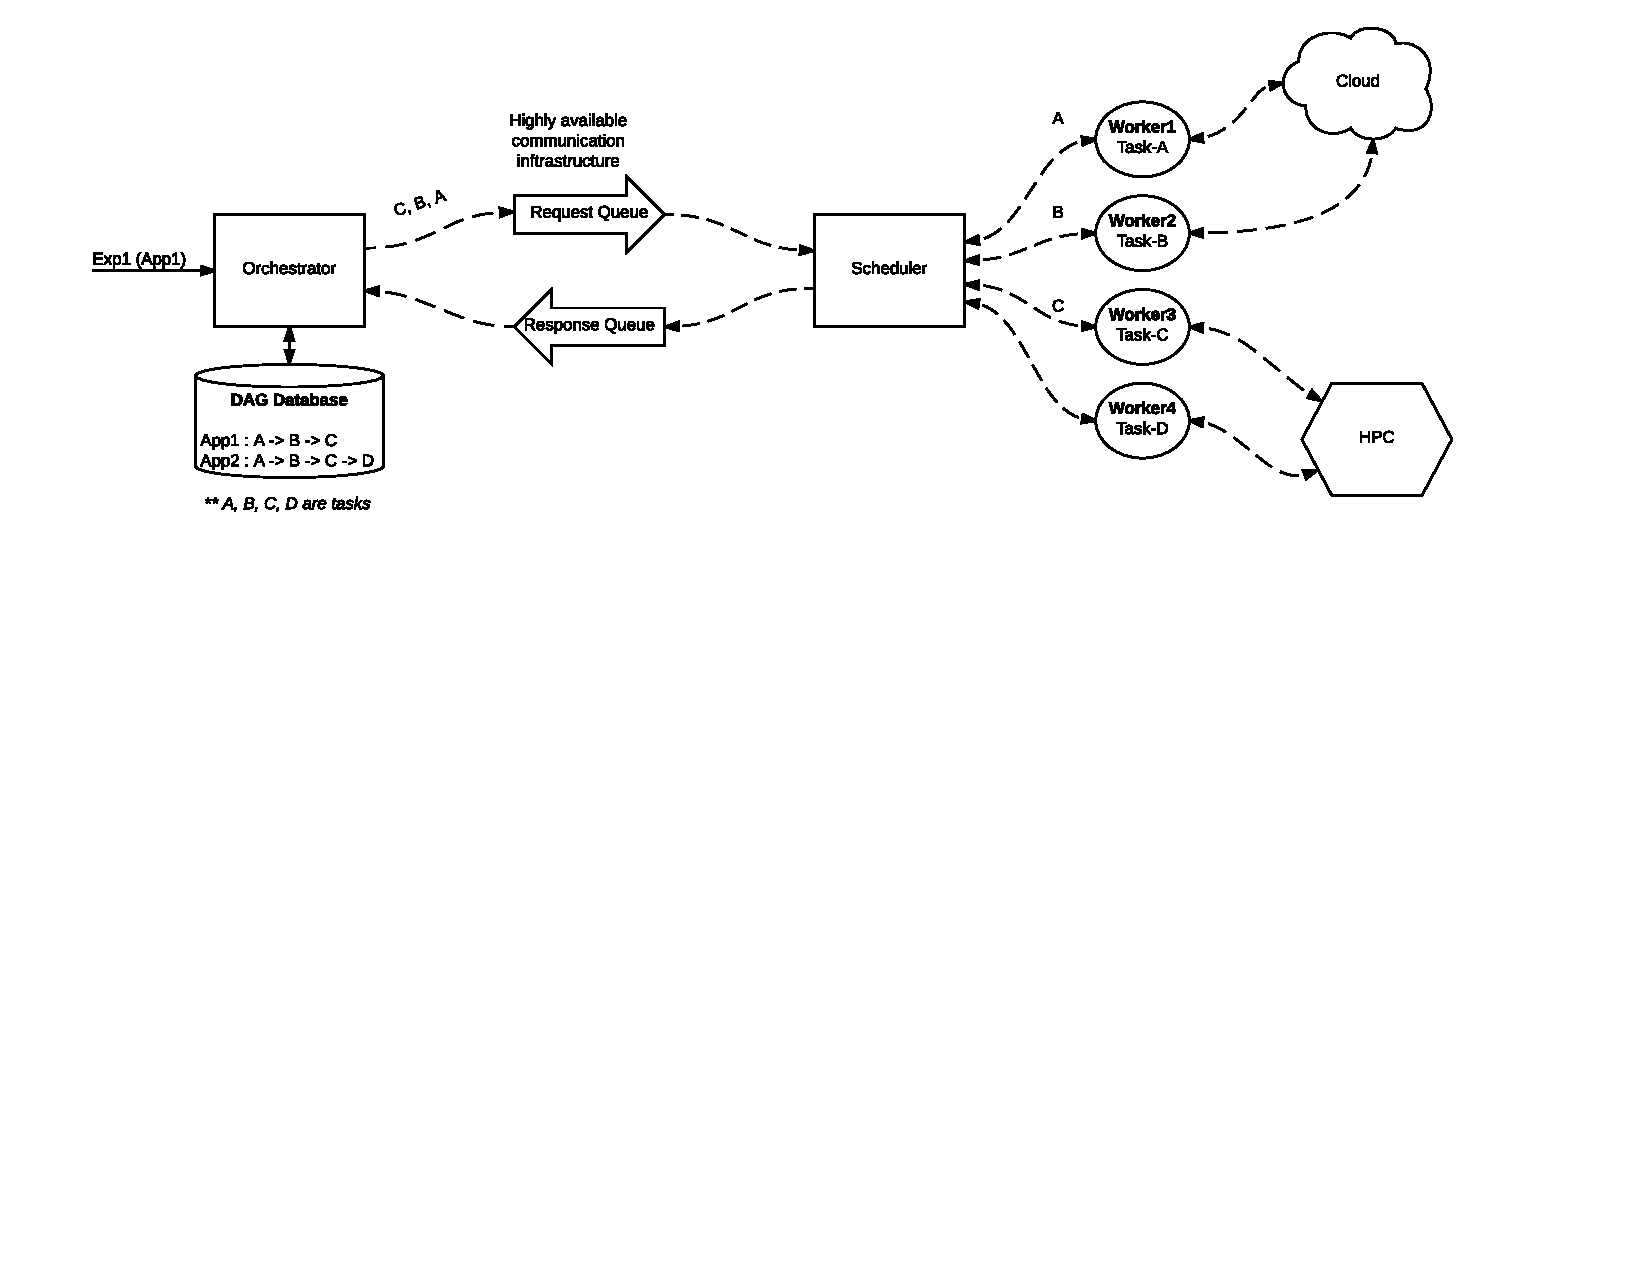
\includegraphics[height=3in, width=7in]{figures/overall-design.pdf}
\caption{A sample black and white graphic
that needs to span two columns of text.}
\end{figure*}

There are 2 concerns which arise here:
?	How does the scheduler know/decide which worker to pass on the task execution to?
?	How do we upgrade a worker, say with a new task ?E? implementation, in such a manner that if something goes wrong with code for ?E?, the entire worker node should not fail? In short, avoid regression testing the entire worker module.
To address the first problem, we suggest to use a paradigm similar to how Apache Aurora agents (workers) report available capabilities to the Aurora master (scheduler). In Aurora, the slave nodes constantly report back to the master how much processing power they have; and accordingly, the master decides which slave to pass a new job request to. In our case, we can have the workers advertise to the scheduler which tasks they are capable of executing and the scheduler acts accordingly.
To address the second concern, we suggest to have the task implementations bundled in separate JARs, so that if there is a problem with one task the others don?t get affected and can be ?repaired? without impacting other existing tasks impls. There might be better ways to do this, but this is what I could think of right now.
As mentioned before, adding a new task implementation ? which will need upgrades to all workers will be easy and hassle-free as each worker will report back to the scheduler their capability to handle that new task, as and when upgrade finishes (incremental upgrade). Having a custom scheduler also provides us other benefits such as:
?	Handling corner cases ? eg: task execution on one worker fails (for some unforeseen reason), then the scheduler can retry it on a different worker.
?	Prioritize experiments ? scheduler higher priority experiments before normal priority ones (I just made this one up).

\subsection{Other Designs}

\section{Validation of the design}

\section{IMPLEMENTATION \& EVALUATION}

\section{RELATED WORK}

HTCondor \cite{htcondor} architecture is very similar to our proposed design, it gives robust workload management system for compute-intensive jobs. It provides job queueing mechanism, scheduling, priority scheme, monitoring, and resource management.
HTCondor employees matchmaking algorithm to schedule job on particular node. It uses ClassAd mechanism for matching resource requests (jobs) with node. Whenever job is submitted to Condor, it states both requirement and preferences, such as required memory, name of the program to run, user who submitted the job and a rank for the node that will run the job. On the other hand, nodes advertise their capacities in terms of RAM, CPU type and speed, current load with other static and dynamic properties.
Scheduler continuously read all the job ClassAds and all the node ClassAds and ensures that the requirement in both ClassAds are satisfied before scheduling any job on a node. HTCondor can be used to build highly scalable Grid-style computing environment, it makes use of cutting edge Grid and Cloud-based computing designs and protocols.
HTCondor can be used to build Grid-style computing environments that cross administrative boundaries. 

?	 Actor-Director Models
AKKA uses Actor-Director model to provide elegant solutions in distributed environment. Essentially, Actor model employees lightweight event-driven processes to provide robust platform for applications. It raises abstraction level by hiding low level non- blocking I/O, concurrency, parallelism and distribution. AKKA provides strong set of APIs for java and scala to control lifecycle of the actors. 

\subsection{}

\section{Conclusions}

In current capacity, implemented prototype supports pull mechanism between scheduler and workers. Here, we are depending on messaging infrastructure (RabbiMQ) for delegating tasks to workers. This approach works fine but as we move ahead system might need to absorb surprising business wants, considering this, it is better to have more control over task delegation rather than depending on third party technologies. The push mechanism would give better control over workers and task execution. Onc can think of using matchmaking algorithm used by HTCondor here, workers can advertise their capacities in terms of tasks capabilities, available memory, current load, CPU speed etc, scheduler can do match tasks requirements with available worker and assigns task to particular worker. That way scheduler knows where each task is executing. Also, scheduler can monitor node heartbeats to maintain workers states and can spin up new instances as required. As mentioned earlier one can think of gossip protocol to communicate state and resource information. Serf is a widely used gossip protocol with support for scalability and fault tolerance. 
Also, in this prototype we have used RabbitMQ \cite{rabbitmq} for communication between Orchestrator and Scheduler as well. Considering, it could be a single point of failure once can think using more robust, scalable and fault tolerant messaging infrastructure. Kafka is a good contender, we are planning to replace RabbitMQ with the same.    

%\begin{acks}
%  The authors would like to thank Dr. Yuhua Li for providing the
%  matlab code of  the \textit{BEPS} method. 
%
%  The authors would also like to thank the anonymous referees for
%  their valuable comments and helpful suggestions. The work is
%  supported by the \grantsponsor{GS501100001809}{National Natural
%    Science Foundation of
%    China}{http://dx.doi.org/10.13039/501100001809} under Grant
%  No.:~\grantnum{GS501100001809}{61273304}
%  and~\grantnum[http://www.nnsf.cn/youngscientsts]{GS501100001809}{Young
%    Scientsts' Support Program}.
%
%\end{acks}

\bibliographystyle{ACM-Reference-Format}
\bibliography{distributed-task-execution} 

\end{document}
